\section{Nine priced corrections}
\label{app:defects} Each of the following was found by re-reading committed artifacts, not by
running new experiments. Items 1--5 were harness defects, the measurement
itself was contaminated. Items 6--8 were claims withdrawn after correction
the measurement was sound, but the claim drawn from it was not. Item 9 is
the AR-30B gold-leak, found the same way as the first eight. Six of
the nine biased against the autoregressive arm. \begin{enumerate}
\item \textbf{Decoding configuration.} Qwen's checkpoint sets
\texttt{repetition\_penalty}\,$=$\,1.1, which suppresses span-copying and
empties the \texttt{host} field. Correcting to 1.0 moved the dense AR-1.5B's
12-field F1 from \defectOneFBefore{} to \defectOneFAfter\ ($n{=}2000$).
\emph{Against AR.} \item \textbf{Serving parity.} AR ran a naive HuggingFace generate
loop while DG ran on vLLM~\cite{vllm2023} with continuous
batching. Moving the dense AR-1.5B to vLLM moved its p50 from
\defectTwoBefore{} to \defectTwoAfter\,ms (\defectTwoRatio$\times$,
$n{=}2000$), erasing a diffusion lead that had looked like a factor of four.
\emph{Against AR.} \item \textbf{Parser policy.} At $L{=}512$, \rambleRate\% of AR outputs
contained multiple JSON objects. The old parser took the last (most-drifted)
copy; first-object-wins moved the dense AR-3B's 12-field F1 from
\defectThreeBefore{} to \defectThreeAfter. \emph{Against AR.} \item \textbf{Metric defaults.} The completeness metric treated falsy values
(\texttt{""}, \texttt{0.0}, \texttt{False}) as missing keys. AR
emits falsy defaults on early stop; DiffusionGemma always fills every field.
Distinguishing absent from present-but-falsy moved AR completeness from
\defectFourBefore\% to \defectFourAfter\%. \emph{Against AR.} \item \textbf{Provenance.} A CLI default wrote an AR model name into three
\LLaDA\ result files (the perturbation, refinement and bounded-deadline runs).
Biases no comparison but made audit impossible until correction
sidecars were written. \emph{Neutral.} \item \textbf{Classical-parser baseline.} An earlier draft claimed a classical
parser matched LLM extraction at 9-field F1 of $0.68$ against $0.85$. What was
recorded as a near-match was self-grading: our ``Drain'' was a regex fallback
instead of the reference implementation~\cite{drain}, and the gold generator
was the same code. The claim is withdrawn. \emph{Neutral} (inflated a third baseline, not
either architecture). Found by re-reading the gold-generation script. \item \textbf{Contaminated semantic gold.} An earlier draft claimed structural
and semantic fields separate cleanly, on a 12-field macro where AR led DG by
\twelveGap\ F1. The semantic gold labels were placeholder output of the same
parser, one a constant across 2{,}000 events. On the decontaminated 9-field
macro the two differ by \qualityGap. The contamination inflated the arm that
fills fields with plausible text (AR) and penalised the arm that leaves them
empty (DG). \emph{Against DG.} Found by re-reading the gold labels. \item \textbf{Queueing model.} An earlier draft claimed an M/D/1 queue
predicts diffusion latency under load. The match was to the measured
saturation knee under Poisson arrivals; under bursty (MMPP) arrivals, which is
what log streams actually produce, the model stops being predictive. The claim
is withdrawn. \emph{Against AR} (overstated how well DG's load behaviour is
modelled).
\item \textbf{AR-30B gold-leak.} The AR-30B harness read its model input
from the gold record file (\texttt{bgl.jsonl}) instead of the raw log
file (\texttt{bgl.raw}), prompting the model with the answer it was
supposed to extract. Combined with \texttt{enforce\_eager} (CUDA graphs
off), vLLM 0.11.0 (vs the pinned 0.25.1), a batched-throughput result
labelled as serial, and a \texttt{Record(**kwargs)} constructor that
silently emptied every prediction (yielding F1\,$=$\,1.0 from
empty-vs-empty scoring), the AR-30B appeared to decode at
48\,ms/token ($7.6\times$ the dense AR-3B's 6.3) and scored perfect
quality. Re-measured on the pinned stack with the corrected harness:
7.2\,ms/token, F1\,$=$\,0.870. The headline ratio moved from
$15.6\times$ to $2.5\times$, the crossover from $L^{*}\!=\!6$ to
$L^{*}\!=\!48$, the batch multiplier from $77\times$ to $25\times$, and
the annual cost gap from \$26{,}000 to \$2{,}600.
\emph{Against AR} on latency (the eager mode and old engine inflated
AR's decode cost); \emph{Against DG} on quality (the gold leak
inflated AR's F1 to 1.0). The latency effect dominated the headline.
Found by re-reading committed artifacts, the same method as the first
eight. A recurrence guard now rejects any input to
\texttt{build\_chat\_messages} that parses as a gold JSON record, and
\texttt{verify\_numbers.py} fails on any cited artifact lacking
provenance.
\end{enumerate} The clustering on one arm is not a coincidence: a comparison harness written by
someone hoping the new architecture wins fails asymmetrically, because the
arm the experimenter is not rooting for inherits the checkpoint defaults, the
naive serving path, and the mature production infrastructure.
Figure~\ref{fig:defects} prices all eight.

\begin{figure}[ht!]
\centering
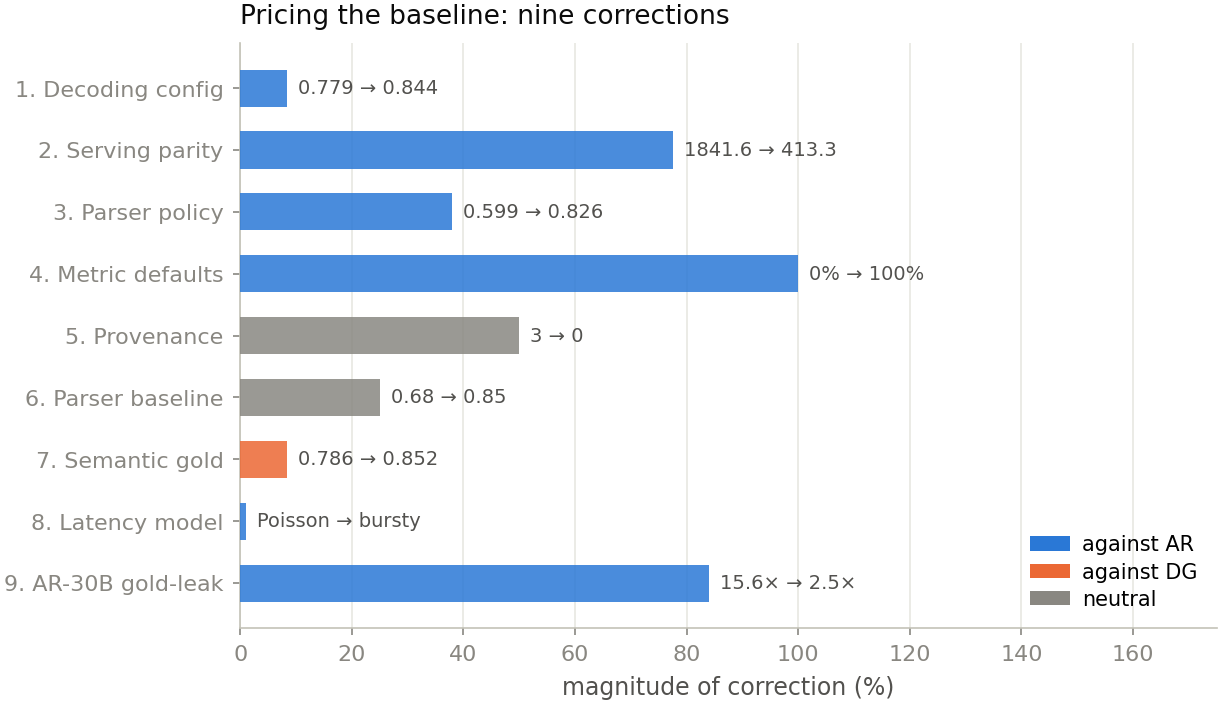
\includegraphics[width=\linewidth]{figures/fig8_defects.png}
\caption{Nine priced errors in our own comparison harness, each found
by re-reading committed artifacts (BGL, $K{=}8$). Six of nine biased
against the autoregressive arm, the harness flattered the
architecture we were hoping would win. Arms and sample sizes differ by
correction: 1 and 2 are the dense AR-1.5B ($n{=}2000$), 3 and 7 the
dense AR-3B ($n{=}300$), 4 is LLaDA-8B ($n{=}200$--$500$). Bar length
is the magnitude of each correction in its own units (F1 delta,
latency ratio, or percentage points), so bars are comparable within a
correction, not across them.}
\label{fig:defects}
\end{figure}
